
\subsection{Long-memory order flow and observation-clock morphology}
\label{app:stylised-facts-recovery}

Figure~\ref{fig:stylised-facts-recovery} separates two mechanisms that can
otherwise be confused.  The operational solver produces one completed pair of
price paths on the fixed grid.  Its innovations are Gaussian, while the
declared market-order signs are an exogenous order-splitting input.  Independent
book-specific renewal clocks are then applied by the exact previous-refresh
map in Eq.~\eqref{eq:subordination}.  Thus ``Gaussian'' labels the operational
innovations and never a waiting-time distribution.

For each primitive path and book, signs are constant over iid meta-order run
lengths $L$ with tail exponent $\nu=1.5$ and minimum run length two events;
successive run signs are iid and symmetric.  In the corresponding ideal
renewal construction the sign covariance decays as a power law proportional
to $k^{1-\nu}$.  This is a declared long-memory input motivated by order
splitting, not an endogenous consequence of the order-book dynamics and not an
empirical calibration.

The four rows hold the operational dynamics, event tape and query grid fixed.
They differ only in observation:
\begin{enumerate}
\item the completed operational path itself;
\item exponential waiting intervals with rate $0.1\,\mathrm{s}^{-1}$;
\item Mittag--Leffler waiting intervals with $\beta=0.8$ and
  $\tau=10\,\mathrm{s}$; and
\item the exact exponential tilt of that Mittag--Leffler law with
  $\lambda_T=0.0125\,\mathrm{s}^{-1}$.
\end{enumerate}
The resulting zero-return proportions at the five-second query scale are,
respectively, $0$, $0.6063$, $0.9097$ and $0.6648$.  The central spike, QQ
plateau and apparent tail thickening therefore measure observation-clock
morphology.  Untempered subdiffusion produces the longest holds; tempering
reduces, but does not remove, that effect.  A constant finite-horizon sampled
series is retained in distribution and impact averages, but its undefined ACF is not assigned an artificial value. Group ACFs require both books and both antithetic partners to be defined. At the longest horizon, the Mittag--Leffler row has between 121 and 125 of 128 valid groups, depending on lag and observable; this conditional availability is distinct from the unconditional return distribution.

\begin{figure}[p]
\centering
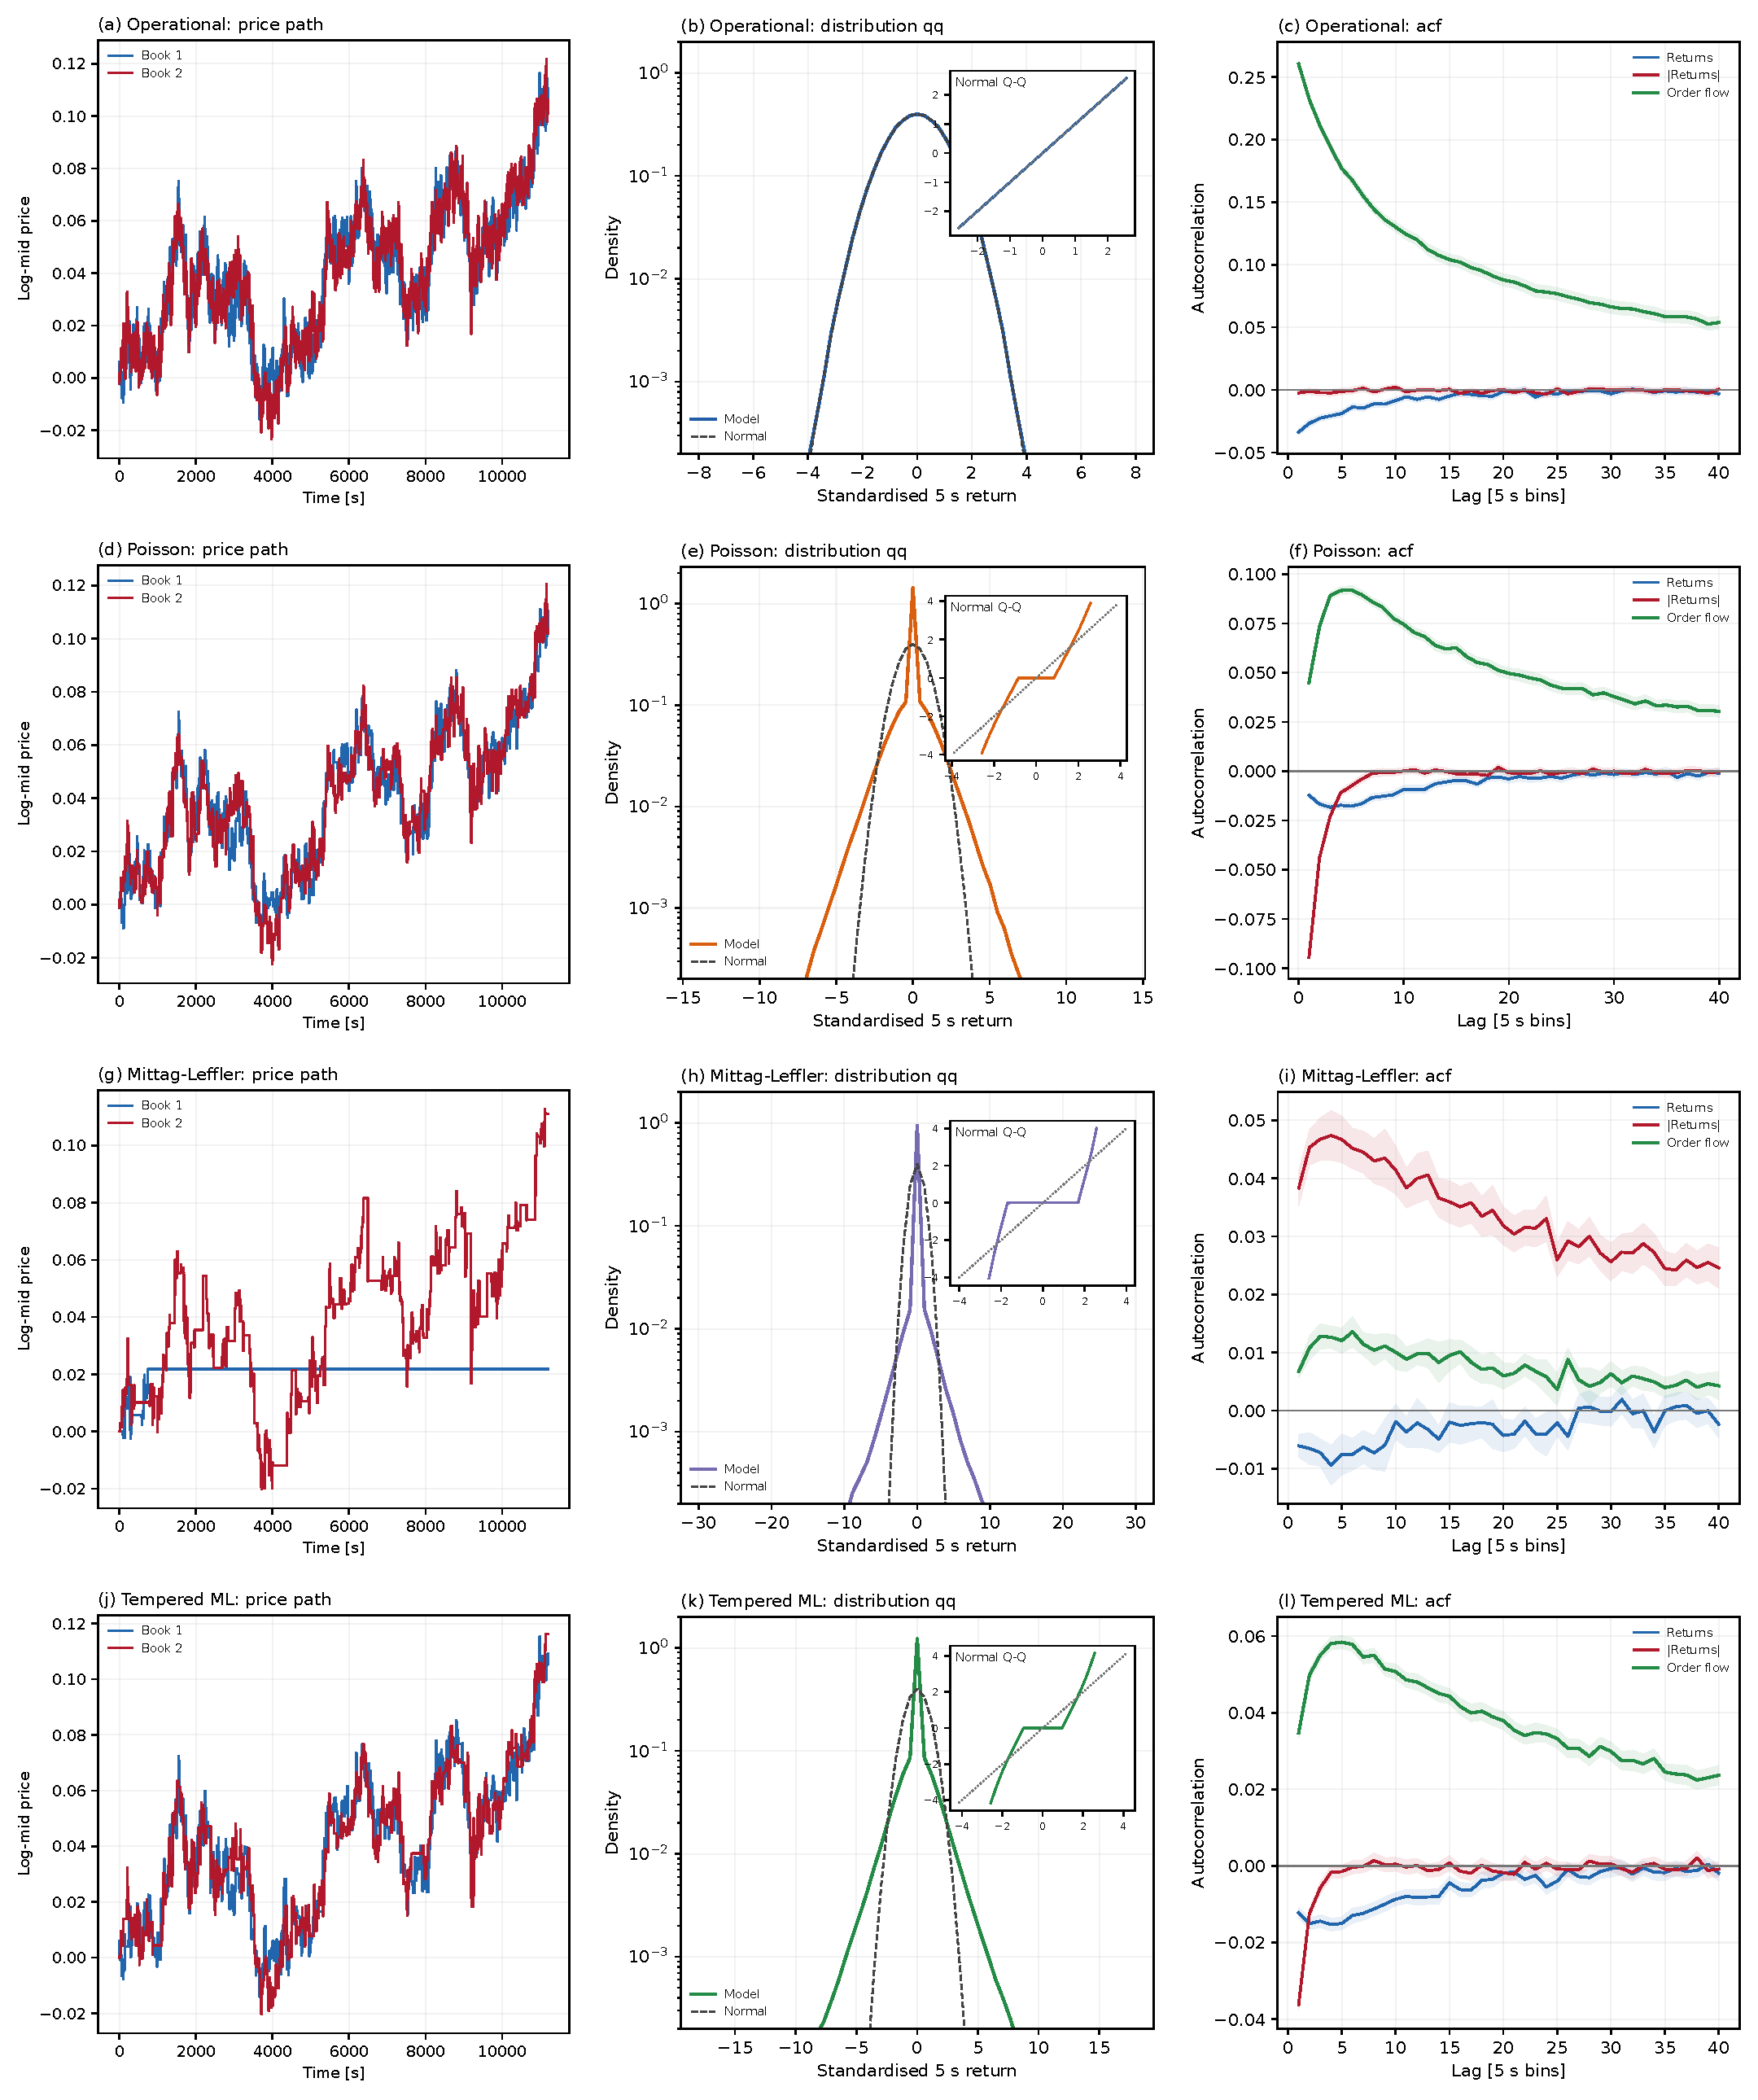
\includegraphics[width=\textwidth,height=0.74\textheight,keepaspectratio]{figures/figure-13-stylised-facts-recovery-v2.pdf}
\caption{\textbf{Operational long-memory input and observation-clock morphology.} The four rows show operational, Poisson, Mittag--Leffler and tempered Mittag--Leffler observation. The left column is the predeclared primitive group-2 path, with blue/red denoting books 1/2. The centre column shows pooled standardized five-second return densities on a logarithmic scale, with a fixed normal reference and QQ insets. The right column shows return (blue), absolute-return (red) and declared-flow (green) ACFs at lags in five-second bins; shading is pointwise 95\% mean uncertainty. Summaries use 128 independent groups with explicit antithetic partners, 22400 half-second steps and $\Delta x=0.1$. Exogenous quantity-0.0002 events arrive with probability 0.05 per step and Pareto sign-run exponent 1.5; only the longest horizon has the terminal 149-step no-event margin. Clocks start at time zero. Infinite-mean renewal aging makes observation-window length material. Constant paths remain in densities; undefined ACFs are omitted only at the declared complete-group level. Gaussian innovations do not require Gaussian observed returns, and no tail or clock parameters are refitted.}
\label{fig:stylised-facts-recovery}
\end{figure}
